%#########################################################################################
\chapter{Evaluation}
\label{chap:evaluation}
%#########################################################################################

In the previous chapter, STODaP approach was presented in details, as well as the supporting tools and their implementation choices.
Practical results were also characterized, showing concrete achievements on the open data organization problem.

In this chapter, the evaluation of STODaP server is described.
The system was compared to other mechanisms on the task of searching for open datasets.
We first present a theoretical background on search engine evaluation methodologies in \autoref{sec:lit_review}.
Then, we show the experimental setup in \autoref{sec:setup}, the pre-evaluation procedure in \autoref{sec:pre_evaluation} and the results in \autoref{sec:results}.
Some concluding remarks are driven on the final section.

\section{Methodology Evaluation Background}
\label{sec:lit_review}

As the amount of online available data gets bigger and bigger, search methodologies are increasingly necessary to allow users accessing relevant content.
Thus, it is crucial to develop evaluation techniques that allows researchers to compare different algorithms and find the most adequate ones for each context.

\citeonline{Cheng2010} developed two measures for assessing \emph{user satisfaction} and \emph{user effectiveness} on Interactive Information Retrieval systems.
The first one is called Normalized Task Completion Time (NT), and is calculated as the relation between task completion times for novices and experts.
Following the same reasoning, the Normalized User Effectiveness (NUE) evaluates the relation between relevant documents retrieved by novices and experts, proportional to NT.
Authors claim that this normalization procedure turns the measures more stable against task complexity variations.
Results show that the NT is highly correlated to user satisfaction, while NUE is a better indicator for effectiveness when compared to simple task completion time.
The learning curve was also better explained by NT and NUE than by task completion time.

In a contrary direction, \citeonline{Xu2009} defend the use of task completion time as a robust measure to assess in which extent the search engine helps users to complete a task.
Additionally, these authors found a negative correlation between user satisfaction and task completion time.
An important result of this study is a mathematical development which shows that a cross-over design reduces significantly the variance of the experiment.
Cross-over design means that, when comparing systems A and B on several tasks, every user tests both systems and completes all tasks once, half of them in A, and the other half in B.

%config 1: metade dos usuarios usam um sistema, metade outro, todos fazem todas as tarefas
%config 2: todos fazem todas as tarefas nos dois sistemas > problema : curva de aprendizado - solução - crossover - todos usuarios vao usar os dois sistemas, mas para tarefas diferentes : metade dos usuarios faz metade das tarefas no A e metade no B, e vice-versa

In a survey dealing specifically with faceted search, \citeonline{Wei2013} presents a review about relevance and cost-based metrics on the faceted search context.
Regarding relevance metrics, authors go through a number of works which use precision, recall or F-measure in the same way as on non-faceted search evaluation.
Cost-based metrics look at the time needed to complete a search task, and memory usage.
These metrics were used to compare performance between faceted and non-faceted engines.

Although the Web and search engines have dramatically changed in the last 10 years, the perspective brought by \citeonline{Vaughan2004} is still relevant.
The focus in this work relies on the quality of ranking, i.e., the order in which results are presented.
Both works presented previously rely on the task completion time, which brings with it factors that do not depend on the system, e.g., users ability, and factor not directly related to the search-engine, such as usability.
By looking specifically at the ranking quality, the evaluation methodology may ignore these aspects, and keeps full attention on the search mechanism.
In this work, author proposes non-binary counterparts to the traditional precision and recall measures, with the intention of adding human relevance judgement aspects to the evaluation.
Specifically, two measures are proposed: (i) \emph{Quality of result ranking}, as counterpart of precision and (ii) \emph{Ability to retrieve top ranked pages}, as counterpart measure of recall.
Both measures rely on a human driven ranking of results, which is correlated with the search engine one in the first case.
The second measure evaluates in which extent the top-results are present in each search engine, for the same query.

\section{Experimental Setup}
\label{sec:setup}

-- hiposteses e metricas

% \citeonline{Cheng2010}
% entry questionaire to make sure the users were able to make the test
% novices received a basic training, reading instructions and questions we answered
% The researchers ran a pilot study before finalizing the search tasks to make sure that LexisNexis Academic could retrieve the relevant documents for all these search tasks. Each
% For each search task, the subject stopped the search session when either the information need was satisfied or he or she gave up the task. The researchers observed the subjects performing their searches in order to ensure that the correct procedures were being followed. The researchers also recorded the task completion time of each task, and asked the subjects to answer a questionnaire after each task. As
% 4. Task completion time (T): The time from the start until the completion of a retrieval task. The task completion time is recorded in seconds, but note that the minute was the unit in the calculations. The subjects stopped each search session by themselves, either once their search needs were satisfied or when they gave up.
% 5. User satisfaction (S): An ordinal number indicating the level of user satisfaction. A questionnaire was provided to the users after each search was complete. It asked the subjects to rate their satisfaction level towards the system in regard to supporting the accomplishment of the search task, using a scale from 1 (not satisfied at all) to 5 (extremely satisfied).

In this section, we describe in details our experimental setup.
First of all, we define the evaluation goals:
\begin{itemize}
	\item When searching for open data, how does STODaP compares to other data-specific and general search engines?
	\item Is the STODaP server an useful tool for searching open datasets?w
\end{itemize}

\subsection{Subjects}

The aim of STODaP server is to facilitate access to open data to the general public.
We consider that experts already have their own strategies and sources for finding adequate data.
Thus, we do not require experience in open data.
However, users must have some previous knowledge on internet navigation. 
Knowledge on basic data processing tools such as spreadsheet processors is also desired, so that subjects can at least imagine a potential use of data.

\subsection{Tasks}

By design, STODaP server is a tool for interlinking different Open Data Portals.
Thus, in this evaluation we aim to assess the ability of gathering similar information from several ODPs, rather than finding specific datasets on the Web.

The evaluation tasks where selected based on: (i) topic relevance of datasets on the open data community, based on criteria defined by Open Data Index\footnote{http://index.okfn.org/} (ii) the existence of search results on STODaP server.
This restriction allows us only to make assertions about the performance of STODaP server on the topics covered by the system, which consists of large base of open data portals, as described in \autoref{sec:stodap_architecture}.
Broader conclusion would require large scale evaluations, which are over the scope of this thesis.
Defined tasks are:

\begin{itemize}
	\item Find open datasets containing 2015 budget data from locations in 5 different countries.
	\item Find open datasets containing procurement information in 3 different idioms.
	\item Find open datasets about Water Quality on 7 different rivers.
\end{itemize}

\section{Procedure}

The following procedure was driven during the evaluation process:

\begin{itemize}
	\item Participants filled the entry-questionnaire (5 minutes);
	\item The main idea of the project was explained, followed by an explanation about (10 minutes)
	\item Participants were assigned numbers and asked to enter this number on the form. 
	\item Three tasks were sequentially presented. 
	Each one was demanded to be completed either using STODaP server, the Exversion Data Search Engine\footnote{Available at \url{https://www.exversion.com/search/}} or conventional search engines \cite{Xu2009}.
	The combination between search method, task and ordering was randomly chosen for participants.
	\item For each task, the challenge was presented with the appropriate number of text fields for pasting the results links.
	\item The time taken for each task was automatically calculated. The search string used in STODaP server were also captured.
	\item An evaluation questionnaire was filled by the subjects, containing questions about usability and satisfaction.
\end{itemize}

\subsection{Validation}
Each entry-questionnaire was analysed in order to determine if it is valid to our evaluation, in terms of internet experience.

The answers were also checked in order to confirm if the dataset links provided are really valid answers to the assigned task.


%#######################################
\section{Pre-Evaluation}
\label{sec:pre_evaluation}
%#######################################

In order to test and adjust our evaluation setup, we ran the process described above with a group of seven students of an Information Retrieval graduate course, at the Federal University of Rio de Janeiro, on the 12th of July 2016.
The results of this evaluation round can be seen in \autoref{tab:pre_eval_questionnaire} and \autoref{tab:pre_eval_results}.
Although the main target of this pre-evaluation process was to assess the evaluation procedure (and not the STODaP server), it is useful to look at the results to have the first impressions.

\begin{table}[h]
\ABNTEXfontereduzida
\centering
\caption[Answers to the entry and evaluations questionnaires.]{Answers to the entry and evaluations questionnaires. The first four questions correspond to the entry-questionnaire, applied before the evaluation. The two remaining questions were answered after completing the evaluation tasks. Task Completion Time (TCT) is the average number of seconds taken to finish the task. Accepted answers is the percentage of answers considered valid, over a total of 15.}
\label{tab:pre_eval_questionnaire}
\begin{tabular}{|>{\centering\arraybackslash}m{.5cm}|>{\centering\arraybackslash}m{.7cm}|>{\centering\arraybackslash}m{1.cm}|>{\centering\arraybackslash}m{.8cm}|>{\centering\arraybackslash}m{.8cm}|>{\centering\arraybackslash}m{2cm}|>{\centering\arraybackslash}m{2.9cm}|>{\centering\arraybackslash}m{2.4cm}|>{\centering\arraybackslash}m{1.3cm}|}
\hline
& 	Age & Internet Ability (1 - low; 5 - high) & Data Ability (1 - low; 5 - high) & Open Data Ability  (1 - low; 5 - high) &	Do you think STODaP is a useful tool for finding data on the web?  (1 - not useful; 5 - very useful) &	How easy is it was get the data you need using the STDOaP in comparison with the other methods?  (1 - harder; 5 - easier) & 	Average TCT (seconds) & Accepted Answers (\%)\\ \hline
1& 	27& 	5& 	3& 	1& 	4& 	2& 	295.7 +/- 98.8 & 100 \\ \hline
2& 	23& 	5& 	4& 	3& 	5& 	3& 	833.3 +/- 151.8 & 80 \\ \hline
3& 	27& 	5& 	5& 	5& 	2& 	2& 	560.0 +/- 103.2 & 33 \\ \hline
4& 	23& 	5& 	4& 	3& 	5& 	4& 	845.0 +/- 523.9 & 73 \\ \hline
5&	26& 	5& 	3& 	2& 	5& 	5& 	625.3 +/- 269.5 & 67 \\ \hline
6& 	29& 	5& 	5& 	3& 	4& 	4& 	527.0 +/- 287.5 & 100 \\ \hline
7& 	22& 	5& 	4& 	1& 	5& 	5& 	351.0 +/- 121.2 & 80 \\ \hline
\end{tabular}
\end{table}

\begin{table}[]
\ABNTEXfontereduzida
\centering
\caption[Task Completion Time of the pre-evaluation test, in seconds.]{Task Completion Time of the pre-evaluation test, in seconds. 
Each cell contains the number of seconds that one or more subjects took to complete the task with the correspondent search method.}
\label{tab:pre_eval_results}
\begin{tabular}{|>{\centering\arraybackslash}m{2.0cm}|>{\centering\arraybackslash}m{2.4cm}|>{\centering\arraybackslash}m{2.4cm}|>{\centering\arraybackslash}m{2.4cm}|>{\centering\arraybackslash}m{2.4cm}|>{\centering\arraybackslash}m{2.0cm}|}
\hline
\textbf{Tasks / Search Methods} & \textbf{Water Quality} & 	\textbf{Budget information} &	\textbf{Procurement} &	\textbf{Average and Standard Deviation} & \textbf{Accepted Answers (\%)} \\ \hline
\textbf{Exversion} &	723, 884, 468 &	235, 382 &	558, 518 &	538.3 +/- 198.5 & 78 \\ \hline
\textbf{STODaP} &	435, 493, 460 &	397, 184, 517, 1048 & -	&	504.9 +/- 244.0 & 83 \\ \hline
\textbf{Free} &	1580 &	702 &	401, 217, 180, 1001, 729 &	687.1 +/- 456.3 & 63 \\ \hline
\textbf{Average and Standard Deviation} &	720.4 +/- 383.7 &	495.0 +/- 276.7 &	514.9 +/- 266.7 & & \\ \hline
\textbf{Accepted Answers (\%)} & 76 & 80 & 71 & & \\ \hline
\end{tabular}
\end{table}

\autoref{tab:pre_eval_questionnaire} shows the answers of each subject to the questions both before and after running the evaluation, together with its average task completion time and the percentage of valid answers.
As expected, all subjects are frequent internet users.
Use of data in daily work or study is also high, but the only one declared himself an open data expert.
Coincidently or not, this subject was the only who did not considered STOaP an useful tool for finding data on the web.
Four out of seven considered that completing the tasks with STODaP was easier than with other methods.
The average Task Completion Time had a huge variation, with a minimum of 295 seconds and a maximum of 845 seconds.
Through a manual procedure, each answer was verified in order to check if it really corresponds to the given task.
The verification was not strict, and answers were discarded only if they were clearly wrong, or blank.
Open data criteria were not taken into account.
No significant correlation was verified between TCT and accepted answers rate.

\autoref{tab:pre_eval_results} shows the Task Completion Times for each task and search method.
We can easily notice that a choosing a random generator for attributing tasks, search methods and orders was a mistake, specially with a small number of rounds.
There were 36 possibilities (6 orderings for tasks $\times$ 6 orderings for search methods) but only 7 rounds were used.
Thus, the number of combinations between tasks and search methods ended up quite unbalanced, and there was no combination of STODaP search method with the procurement task.
Average TCT for tasks and search methods were also calculated.

After running the procedure, a conversation round was driven with the students on order to get insights both about the tool and the evaluation procedure.
The following suggestions and comments were made:

Regarding the evaluations interface:

\begin{itemize}
	\item Alert that search engines should be open in another tab;
	\item Write the tasks more clearly and specific (e.g., asking budget 2015 may include 2014-16?)
	\item On the final questions, positive answers to the system were at the left side, which is not usual and confused some subjects;
	\item State more clearly that only the link to the dataset should be answered;
	\item Makes clear that users are allowed to use auxiliary tools such as translators or Wikipedia in order to better understand the tasks;
	\item State more clearly that users should only look to the dataset title, and there is no need to open it;
	\item Explain that only some specific portals are indexed, not all open data in the world.
\end{itemize}

Regarding the evaluations procedure:
\begin{itemize}
	\item On the evaluation questionnaire, ask the English proficiency and other languages, and ask if the English language hampered the performance;
	\item To few questions - do not evaluate learning curve.
\end{itemize}
	
Regarding the STODaP faceted search interface:
\begin{itemize}
	\item There should be an explanation about faceted search and how does it work;
	\item Regarding the Portal facet, it was suggested to write portals name in spite of url, when this metadata is available
	\item One participant reported that he took a while to realize the language facet; after seeing it, it was very quick.
	\item It was suggested to include the possibility of making the query broader by including facets with OR.
\end{itemize}	

There were some positive comments:
\begin{itemize}
	\item It was noted that results presented by STODaP had a higher quality in relation to Exversion, mainly because the latter automatically uses an OR logic between two terms.
	This results in many unwanted outputs.
	\item The possibility of searching English keywords and getting multi-language results was also positively mentioned, because no other tool presents such feature.
	\item The STODaP interface, in its search results, exhibits datasets with all its tags.
	This was positively noted, because it helps to decide quicker if a dataset is of interest or not.
\end{itemize}	

Analysing students while they were completing their tasks was also show some new perspectives.
It was noticed that some subjects tried to look deep at datasets in order to verify if they met the task criteria.
It should be harder stressed in the explanation that this is not necessary, since the our objective is only to find dataset, and not to verify their quality.
Some students tried to use analytic tools such as Google Public Data.
Their focus is rather on analysing (open) data sets than on making them available for download in machine readable formats.
Thus, for our intentions, this is not considered open data and it should also be stated in the explanation.

After considering the above mentioned comments, the procedure was enhanced and applied to the main groups.
Results are described bellow.

\section{Results}
\label{sec:eval_results}

In this section, we describe the application of the evaluation procedure and present the results achieved.

In our experiment, participants were first year university students attending a class on the topic Introduction to Information Systems, at the Federal University of Rio de Janeiro, in Brazil.
An entry-questionnaire was filled by the participants, whose answers are summarized in \autoref{tab:eval_summary}.
Participation was not mandatory and non identified, and there was no reward for participants.

\begin{table}[]
\ABNTEXfontereduzida
\centering
\caption{STODaP evaluation - summary of subjects profile}
\label{tab:eval_summary}
\begin{tabular}{|p{8cm}|p{2cm}|}
\hline
Participants & 18 \\ \hline
Age & 20.5 \\ \hline
Internet knowledge (1 - Never Used; 5 - Always use) & 5\\ \hline
Use of data (1 - I've never used any data processing tool; 5 - I'm an expert in advanced data processing tools) & 2.7\\ \hline
Open Data Experience (1 - Never heard about; 5 - I work often with open data) & 2.3 \\ \hline
English Proficiency (1 - Low; 5 - High) & 4.3\\ \hline
\end{tabular}
\end{table}

The average age of the 18 participants was 20.5 years.
Although all of them use internet every day, direct experience with data processing is low, as well as with open data.
As our tool is developed for non-experts, this sample is adequate to the experiment.

After filling the entry questionnaire, subjects were presented 3 combinations of tasks and search methods.
The resulting URLs were pasted in the appropriated fields and the task completion time was automatically calculated for every task of every subject.
A screenshot of the evaluation tool is shown in \autoref{fig:eval_screenshot}. 

\begin{figure}[h!]
\begin{center}
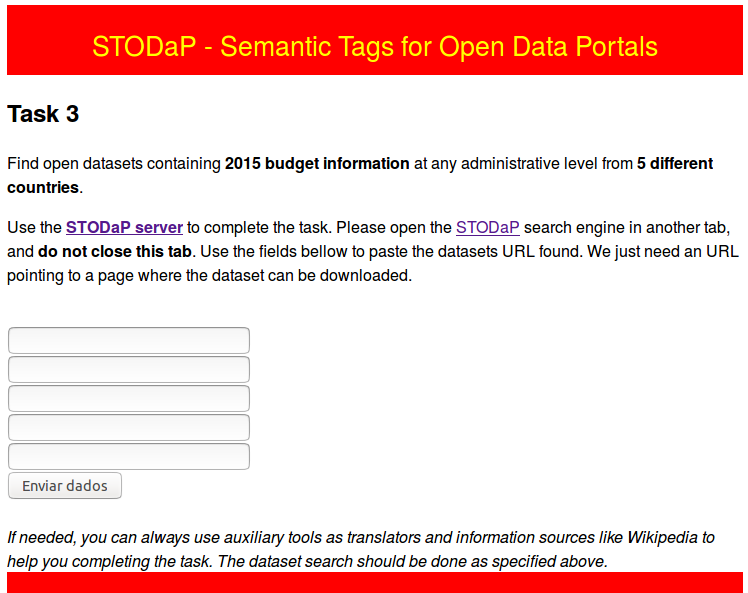
\includegraphics[width=\columnwidth]{images/eval_screenshot.png}
\caption[Evaluation]{Evaluation}
\label{fig:eval_screenshot}
\end{center}
\end{figure}

\subsection{Task Completion Time Analysis}

Task completion time for all subjects is shown in \autoref{tab:eval_results}.

...

\begin{table}[h!]
\ABNTEXfontereduzida
\centering
\caption[Task Completion Time of the evaluation, in seconds.]{Task Completion Time of the evaluation, in seconds. 
Each cell contains the number of seconds that one or more subjects took to complete the task with the correspondent search method.}
\label{tab:eval_results}
\begin{tabular}{|>{\centering\arraybackslash}m{2.4cm}|>{\centering\arraybackslash}m{2.4cm}|>{\centering\arraybackslash}m{2.4cm}|>{\centering\arraybackslash}m{2.4cm}|>{\centering\arraybackslash}m{2.4cm}|>{\centering\arraybackslash}m{2.0cm}|}
\hline
\textbf{Tasks / Search Methods} & \textbf{Water Quality} & 	\textbf{Budget information} &	\textbf{Procurement} &	\textbf{Average and Standard Deviation} & \textbf{Accepted Answers (\%)} \\ \hline
\textbf{Exversion} &	723, 884, 468 &	235, 382 &	558, 518 &	538.3 +/- 198.5 & 78 \\ \hline
\textbf{STODaP} &	435, 493, 460 &	397, 184, 517, 1048 & -	&	504.9 +/- 244.0 & 83 \\ \hline
\textbf{Free} &	1580 &	702 &	401, 217, 180, 1001, 729 &	687.1 +/- 456.3 & 63 \\ \hline
\textbf{Average and Standard Deviation} &	720.4 +/- 383.7 &	495.0 +/- 276.7 &	514.9 +/- 266.7 & & \\ \hline
\textbf{Accepted Answers (\%)} & 76 & 80 & 71 & & \\ \hline
\end{tabular}
\end{table}

% \begin{itemize}
% 	\item Task completion time for each search method (and variance) \cite{Xu2009}
% 	\item Task completion time for each task (and variance) \cite{Xu2009}
% 	\item Correlation between satisfaction and completion time for STODaP server \cite{Xu2009}
% 	\item Correlation between results found in the different search methods \cite{Vaughan2004}
% \end{itemize}

\subsection{Correlation Analysis}

In order to check the correlation between characteristics of the subjects, their evaluation of the tool and their performance on the tests we calculate the correlation coefficient between every variable related to the subjects, i.e.: (i) profile variables such as age, English proficiency, and internet, data and open data abilities; (ii) evaluation about the tool, i.e.: perceived usefulness and usability in relation to other search methods; and (iii) test performance, i.e.: total tasks completion time and percentage of accepted answers.

\autoref{tab:correlations} shows the results.
Age is measured in years. The six following columns are variables that scale from 1 to 5, where 1 worse option, and 5 the better.
Task Completion Time is the sum of time, in seconds, taken to complete all 3 tasks, and the last column is related to the percentage of correct answers.
For this analysis, we considered only subjects with more than 50\% of correct answers.
This filtering was necessary to eliminate some subjects who finished the evaluation very quickly, leaving most of the fields blank.

\begin{table}[]
\ABNTEXfontereduzida
\centering
\caption[Correlation analysis of the results.]{Correlation analysis of the results.}
\label{tab:correlations}
\begin{tabular}{|>{\centering\arraybackslash}m{3.0cm}|>{\centering\arraybackslash}m{1.0cm}|>{\centering\arraybackslash}m{1.0cm}|>{\centering\arraybackslash}m{1.0cm}|>{\centering\arraybackslash}m{1.0cm}|>{\centering\arraybackslash}m{1.0cm}|>{\centering\arraybackslash}m{1.0cm}|>{\centering\arraybackslash}m{1.0cm}|>{\centering\arraybackslash}m{1.0cm}|>{\centering\arraybackslash}m{1.0cm}|}
 \hline
 & Age & Internet Ability &	English Proficiency & Data Ability & Open Data Ability & Usefulness &	Usability &	Task Completion Time &	Accepted Answers \\ \hline
Age & 1.0 	& nan 	& 0.28 	& 0.43 	& 0.24 	& -0.06 	& 0.29 	& -0.13 	& 0.21 	\\ \hline
Internet Ability & nan 	& nan 	& nan 	& nan 	& nan 	& nan 	& nan 	& nan 	& nan 	\\ \hline
English Proficiency & 0.28 	& nan 	& 1.0 	& 0.14 	& 0.42 	& -0.4 	& -0.2 	& 0.19 	& 0.44 	\\ \hline
Data Ability & 0.43 	& nan 	& 0.14 	& 1.0 	& 0.05 	& -0.1 	& 0.01 	& -0.41 	& 0.37 	\\ \hline
Open Data Ability & 0.24 	& nan 	& 0.42 	& 0.05 	& 1.0 	& -0.24 	& -0.64 	& -0.07 	& 0.23 	\\ \hline
Usefulness & -0.06 	& nan 	& -0.4 	& -0.1 	& -0.24 	& 1.0 	& 0.36 	& 0.28 	& 0.08 	\\ \hline
Usability & 0.29 	& nan 	& -0.2 	& 0.01 	& -0.64 	& 0.36 	& 1.0 	& 0.27 	& 0.04 	\\ \hline
Task Completion Time & -0.13 	& nan 	& 0.19 	& -0.41 	& -0.07 	& 0.28 	& 0.27 	& 1.0 	& 0.22 	\\ \hline
Accepted Answers & 0.21 	& nan 	& 0.44 	& 0.37 	& 0.23 	& 0.08 	& 0.04 	& 0.22 	& 1.0 	\\ \hline
\end{tabular}
\end{table}

...

\subsection{Qualitative Analysis}

In this subsection, we derive an analysis of the comments received on the evaluation questionnaire.
From the first group -- first year Computer Science students -- 6 out of 18 subjects wrote comments about the system. 
Four of them complained about the user interface, both visually and in terms of usability: ``The user interface is not intuitive nor pleasant. It should be further worked to help the visualization of results.''

One subject assumed



De fato, foi bem mais simples selecionar o conteúdo. Gostei muito da plataforma. Não estou habituado a pesquisar informações dos tipos propostos, mas o tempo necessário na STOPDaP foi consideravelmente menor para conseguir os resultados desejados. Uma única recomendação que eu faria, que provavelmente já deve ter sido mencionada antes, seriam uns toques novos no CSS do site. 

a UI nao e intuitiva ou agradavel, ela deveria ser melhor trabalhada para auxiliar na visualização dos resultados

It's necessary to update this layout. The project is great. Nice job.

you can make a visual upgrade

as perguntas em ingles não foram muito dificeis de entender não, masportugues apareceu

More data is needed. I really wished I could query data as if it were a single data source.


\section{Conclusions}
\label{sec:conclusion}

After proposing an approach for semantic organization of metadata in Open Data Portals in the previous chapter, in this chapter the approach was evaluated.

Evaluation is a crucial part of every scientific work, since without testing, it is impossible to know if the system works as designed, and if it accomplishes the proposed goals.
However, designing and implementing an information system evaluation is a very complex and challenging task.
Isolating the desired variables from other environment influences is nearly impossible, mainly because of the socio-technical characteristic of information systems.
And if we try to select the ideal subjects to perform the ideal tasks, the evaluation itself can become too complex, and chances are high that it gets too distant of reality.
One can be tempted to look for simple cause-effect explanations in complex problems, i.e., involving humans and systems.
However, according to \citeonline{Morin2011}, the world is an inseparable tissue of actions, interactions, feedbacks, determination and chances, an thus it is too simplistic to think in a direct cause-effect explanation for complex systems.

Searching for open datasets is not an everyday task for the absolute majority of the population.
On the other hand, experienced data scientists already know where to find their data, and even if this data is available or not.
With those questions in mind, we designed this evaluation trying to balance specificity and generality in the choice of subjects.
We also tried to balance the specificity of the tasks, so that it would not be too general (``Find open datasets in Brazil'') but also not too specific (``Find the open data set of 2015 budget in Rio de Janeiro'').
Following this reasoning we chose our subjects (Computer Science students that could work one day with open data and Semantic Web researchers that already work with open data), and our tasks (finding datasets on specific themes according to language and geographical limitations).

Results show that ...




